\documentclass[10pt,a4paper,parskip=half]{scrartcl}
\usepackage[utf8]{inputenc}
\usepackage{amsmath}
\usepackage{amsfonts}
\usepackage{amssymb}
\usepackage{mathpazo}
\usepackage{stmaryrd} % Für den Widerspruchsblitz :D
\usepackage[a4paper,
left=3.0cm, right=3.0cm,
top=2.0cm, bottom=2.0cm]{geometry}
\usepackage{fullpage}
\usepackage{tikz}
\usepackage[german]{babel}
\usepackage{enumerate}
\setlength{\unitlength}{1cm}
\newcommand{\N}{\mathbb{N}}
\newcommand{\A}{\mathcal{A}}
\newcommand{\R}{\mathbb{R}}
\parindent 0mm
\author{Tom}
\title{Analysis 2 - Hausaufgabe 3}
\usepackage{color}
\usepackage{listings}
\usepackage{courier}
 \lstset{
         basicstyle=\footnotesize\ttfamily, % Standardschrift
         %numbers=left,               % Ort der Zeilennummern
         numberstyle=\tiny,          % Stil der Zeilennummern
         %stepnumber=2,               % Abstand zwischen den Zeilennummern
         numbersep=5pt,              % Abstand der Nummern zum Text
         tabsize=2,                  % Groesse von Tabs
         extendedchars=true,         %
         breaklines=true,            % Zeilen werden Umgebrochen
         keywordstyle=\color{red},
    		frame=b,         
 %        keywordstyle=[1]\textbf,    % Stil der Keywords
 %        keywordstyle=[2]\textbf,    %
 %        keywordstyle=[3]\textbf,    %
 %        keywordstyle=[4]\textbf,   \sqrt{\sqrt{}} %
         stringstyle=\color{white}\ttfamily, % Farbe der String
         showspaces=false,           % Leerzeichen anzeigen ?
         showtabs=false,             % Tabs anzeigen ?
         xleftmargin=17pt,
         framexleftmargin=17pt,
         framexrightmargin=5pt,
         framexbottommargin=4pt,
         %backgroundcolor=\color{lightgray},
         showstringspaces=false      % Leerzeichen in Strings anzeigen ?        
 }
 \usepackage{caption}
\DeclareCaptionFont{white}{\color{white}}
\DeclareCaptionFormat{listing}{\colorbox[cmyk]{0.43, 0.35, 0.35,0.01}{\parbox{\textwidth}{\hspace{15pt}#1#2#3}}}
\captionsetup[lstlisting]{format=listing,labelfont=white,textfont=white, singlelinecheck=false, margin=0pt, font={bf,footnotesize}}

% new commands for vectors
\newcommand{\vectwo}[2]{\begin{pmatrix}#1\\#2\\\end {pmatrix}}
\newcommand{\vecthree}[3]{\begin{pmatrix}#1\\#2\\#3\\\end {pmatrix}}

% Füllt man nach Spalte und dann nach Zeile. Dann kann man besser von Vektoren kopieren
\newcommand{\mattwotwo}[4]{\begin{pmatrix}#1 & #3\\#2 & #4\\\end {pmatrix}}

\begin{document}
\begin{center}
\textsc{\Large{Analysis 2 - Hausaufgabe 3}} \\
\end{center}
\begin{tabbing}
Tom Nick \hspace{1.4cm}\= 342225\\
Tom Lehmann\> 340621\\
Maximilian Bachl\> 341455
\end{tabbing}
\section*{Aufgabe 1}
\begin{enumerate}[(a)]
\item \ \\
\begin{minipage}{0.50\columnwidth}
Da $r$ im Gegenteil zur Hausaufgabe 2 nicht begrenzt ist, wäre es eine unendliche Scheibe. Diese würde ungefähr so aussehen, würde man versuchen sie zu zeichnen:
\begin{lstlisting}[caption= Mathematica Code für den Graph von h]
ParametricPlot[{{ r Cos[t], r Sin[t]}}, {t, 0, 2 Pi}, {r, 0, 300}, 
 PlotRange -> {{-100, 100}, {-100, 100}}, 
 AxesLabel -> {r, \[CurlyPhi]}]
\end{lstlisting}
\end{minipage}
\begin{minipage}{0.49\columnwidth}
\begin{center}
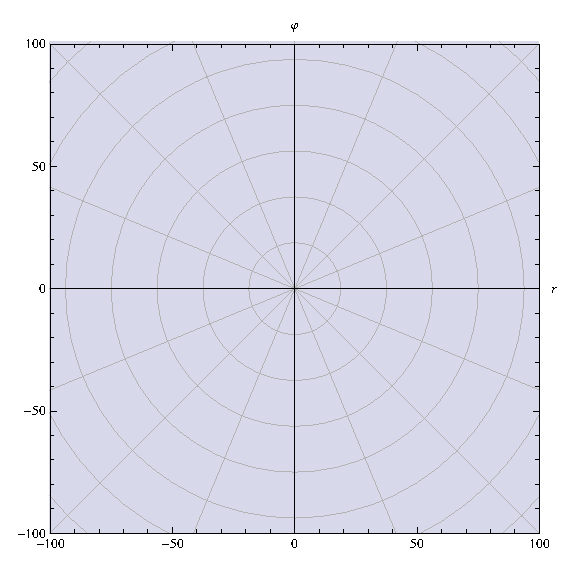
\includegraphics[scale=0.7]{1i.eps} 
\end{center}
\end{minipage}
\item
\begin{align*}
\frac{\partial \vec f}{\partial r}(r, \varphi) &= \begin{pmatrix}\cos(\varphi) \\ \sin(\varphi)\end{pmatrix}\\
\frac{\partial \vec f}{\partial \varphi}(r,\varphi) &= \begin{pmatrix}-r\sin(\varphi) \\ r \cos(\varphi)\end{pmatrix} 
\end{align*}
\item
Die Ableitungsmatrix $\vec {f'}(r ,\varphi)$ ist demnach:
\begin{align*}
\vec {f'}(r, \varphi) &= \begin{pmatrix}\cos(\varphi) & -r \sin(\varphi) \\ \sin(\varphi) & r \cos(\varphi)\end{pmatrix}
\intertext{Für die Determinante gilt deshalb:}
\det(\vec {f'}(r, \varphi)) &= \det \begin{pmatrix}\cos(\varphi) & -r \sin(\varphi) \\ \sin(\varphi) & r \cos(\varphi)\end{pmatrix}\\
&= r\cos^2(\varphi) + r \sin^2(\varphi)\\
&= r \left( \cos^2(\varphi) + \sin^2(\varphi)\right)\\
&= r
\end{align*}
\end{enumerate}
\section*{Aufgabe 2}
\begin{enumerate}[(a)]
\item
Die Komposition $g \circ g$ ist nicht erklärt, da der Urbildraum Elemente des $\mathbb{\R}^3$ verlangt, die Funktionswerte von $g$ jedoch nur aus $\mathbb{\R}$ sind.\\
Die Komposition $g \circ \vec f$ ist erklärt, da sowohl die Funktionswerte von $f$ als auch der Urbildraum von $g$ Elemente des $\mathbb{\R}^3$ sind.\\
Die Komposition $\vec f \circ g$ ist erklärt, da sowohl die Funktionswerte von $g$ als auch der Urbildraum von $f$ Elemente des $\mathbb{\R}$ sind.\\
Die Komposition $\vec f \circ \vec f$ ist nicht erklärt, da der Urbildraum Elemente des $\mathbb{\R}$ verlangt, die Funktionswerte von $\vec f$ jedoch aus $\mathbb{\R}^3$ sind.\item
\begin{align*}
\vec f'(t) &= \vecthree{e^t}{1}{2} \\
g'(\vecthree{x}{y}{z}) &= \left(e^{y-z}, xe^{y-z}, -xe^{y-z}\right)
\end{align*}
\begin{align*} 
(\vec f \circ g)' &= (\vec f' \circ g) \cdot g' \\
&= \vec f'(xe^{y-z}) \cdot \left(e^{y-z}, xe^{y-z}, -xe^{y-z}\right) \\
&= \vecthree{e^{xe^{y-z}}}{1}{2} \cdot \left(e^{y-z}, xe^{y-z}, -xe^{y-z}\right) \ \lightning\ \text{da diese Multiplikation gar nicht möglich ist}
\end{align*}
Hätte man das mit dem Widerspruch auch früher rausfinden können? -- Max
\begin{align*} 
(g \circ \vec f)' &= (g' \circ \vec f) \cdot \vec f' \\
&= g'(\vecthree{e^t}{t}{2t}) \cdot \vecthree{e^t}{1}{2} \\
&= \left(e^{-t}, e^te^{-t}, -e^te^{-t}\right) \cdot \vecthree{e^t}{1}{2} \\
&= \left(e^{-t}, 1, -1\right) \cdot \vecthree{e^t}{1}{2} \\
&= 1 + 1 - 2\\
&= 0\\
g(\vec f(t))' &= 0
\end{align*}
\item
Da wir vorher gezeigt dass das mit $(\vec f \circ g)'$ gar nicht geht, jetzt gleich $(g \circ \vec f)'$:
\begin{align*}
g(f(t))' &= g(\vecthree{e^t}{t}{2t})' \\
&= (e^te^{-t})' \\
&= (e^0)' \\
&= 1' \\
&= 0
\end{align*}
Somit kommt bei beiden Lösungswegen das gleiche Ergebnis heraus.
\end{enumerate}
\section*{Aufgabe 3}
\begin{enumerate}[(a)]
\item
\begin{align*}
e'(x,y) &= (2xy,x^2) \\
f'(x,y) &= (e^xy^2,2e^xy) \\
\nabla(e\cdot f)(1,1) &= f(1,1) \cdot \nabla e(1,1) + \nabla  f(1,1) \cdot e(1,1) \\
&= e \cdot \vectwo{2}{1} + \vectwo{e}{2e} \cdot 1 \\
&= \vectwo{2e}{1e} + \vectwo{e}{2e} \\
&= \vectwo{3e}{3e}
\end{align*}

\item
Ich nehme mal einfach an, dass die Vektoren eigentlich Spaltenvektoren sein sollen, weil sonst hat das ja gar keinen Sinn...
\begin{align*}
\vec g \times \vec h &= \vecthree{xy^2}{0}{\sin (x)} \times \vecthree{y}{x^2}{0} \\
&= \vecthree{-x^2 \sin x}{y\sin x}{x^3y^2} \\
\vecthree{-x^2 \sin x}{y \sin x}{x^3y^2}' &= 
\begin{pmatrix}
-2x \sin x - x^2 \cos x& 0 \\
y \cos x & \sin x \\
3x^2y^2 & x^32y\\
\end{pmatrix}\\
(\vec g \times \vec h)'(0,1) &= \begin{pmatrix}
0 & 0 \\
1 & 0 \\
0 & 0 \\
\end{pmatrix}
\end{align*}
\item
Ich nehme mal einfach an, dass die Vektoren eigentlich Spaltenvektoren sein sollen, weil sonst hat das ja gar keinen Sinn...
\begin{align*}
\vec u \cdot \vec v &= \vectwo{xyz}{y^3} \cdot \vectwo{\sin(x)z}{y^3} \\
&= xyz^2\sin(x) + y^6 \\
(\vec u \cdot \vec v)' &= (xyz^2\sin(x) + y^6)' \\
&= \begin{pmatrix}
yz^2\cos(x) - xyz^2\sin(x) & xz^2\cos(x) + 6y^5 & 2xyz\sin(x)
\end{pmatrix} \\
(\vec u \cdot \vec v)'(2\pi, 2\pi, 2\pi) &= \begin{pmatrix}\pi^3 \over 8 & \frac{\pi^3}{8} + 6 \frac{\pi^5}{32} & 0\end{pmatrix}
\end{align*}
\end{enumerate}
Bitte überprüft das noch, da sind sicher ein paar Fehler irgendwo...
\end{document}